\documentclass[12pt,a4paper]{article}
\usepackage[utf8]{inputenc}
\usepackage[russian]{babel}
\usepackage[OT1]{fontenc}
\usepackage{mathtools}
\usepackage{amsfonts}
\usepackage{amssymb}
\usepackage{enumitem}
\usepackage{alltt}
\usepackage{graphicx}
\usepackage{indentfirst}
\usepackage{caption}
\usepackage{float}
\usepackage{wrapfig}
\usepackage{physics}
\usepackage{multirow}
\usepackage{longtable}
\usepackage{amsmath,amsfonts,amssymb,amsthm,mathtools}
\usepackage{icomma}
\setlength{\parindent}{0.75cm}
\graphicspath{{pictures/}}
\DeclareGraphicsExtensions{.png}
\usepackage[left=15mm,right=15mm,top=2cm,bottom=2cm]{geometry}
\author{Глотов Алексей}
\begin{document}
\newpage
\begin{center}
\footnotesize{{ГОСУДАРСТВЕННОЕ АВТОНОМНОЕ ОБРАЗОВАТЕЛЬНОЕ УЧРЕЖДЕНИЕ}\break
{ВЫСШЕГО ОБРАЗОВАНИЯ}
\break
{\bf {МОСКОВСКИЙ ФИЗИКО-ТЕХНИЧЕСКИЙ ИНСТИТУТ}}
\break
\small{(НАЦИОНАЛЬНЫЙ ИССЛЕДОВАТЕЛЬСКИЙ УНИВЕРСИТЕТ)}}
\break
\hfill \break
\hfill \break
\begin{center}
\normalsize{Кафедра общей физики}
\end{center}
\hfill \break
\hfill \break
\hfill \break
\hfill \break

\begin{center}
\normalsize {Лабораторная работа 2.2.1}
\end{center}
\hfill \break\\
\large{\textbf{Исследование взаимной диффузии газов}}
\end{center}
\begin{flushleft}
\hfill \break
\hfill \break
\hfill \break
\hfill \break
\hfill \break
\hfill \break
\hfill \break
\hfill \break
\hfill \break
\hfill \break
\hangindent=9cm
\normalsize{Преподаватель:}\hfill
\normalsize{доцент Игуманов А.Ю.}\\
\hfill \break
\normalsize{Обучающийся:}\hfill
\normalsize{Глотов А.А} \\
\hfill \break
\end{flushleft}
\hfill \break
\hfill \break
\hfill \break
\hfill \break
\hfill \break
\hfill \break
\hfill \break
\hfill \break
\hfill \break
\hfill \break
\hfill \break

\begin{center}
Долгопрудный \break
 2022
\end{center}
\thispagestyle{empty}
\section{Введение}

\subsection{Аннотация}

Данная работа посвящена изучению процесса диффузии газов в системе, состоящей из двух компонентов (гелий-воздух). Используются следующие методы измерений: анализ и линеаризация графиков зависимостей U(t) и D(P), а также экстраполяция графика D(1/P). Зависимость напряжения на датчиках теплопроводности от времени снимается с помощью компьютизированной установки

\textbf{Цель работы:}  \begin{enumerate}
	\item регистрация зависимости концентрации гелия в воздухе от времени с помощью датчиков теплопроводности при разных начальных давлениях смеси газов;
	\item определение коэффициента диффузии по результатам измерений.
\end{enumerate}

\textbf{Приборы и материалы:} 
\begin {itemize} 
\item измерительная установка
\item форвакуумный насос
\item баллон с газом (гелий)
\item манометр
\item источник питания
\item магазин сопротивлений
\item гальванометр
\item секундомер.
\end{itemize}

\subsection{Теоретические сведения}

Диффузией называют самопроизвольное взаимное проникновение веществ друг в друга, происходящее вследствие хаотичного теплового движения молекул. При перемешивании молекул разного сорта говорят о взаимной (или концентрационной) диффузии.

Диффузия в системе, состоящей из двух компонентов $ a $ и $ b $ (бинарная смесь), подчиняется закону Фика: плотности потока компонентов $ j_{a,b} $ (количество частиц, пересекающих единичную площадку в единицу времени) пропорциональны градиентам их концентраций $ \nabla n_{a,b}$, что в одномерном случае можно записать как

\[ j_a = -D\frac{\partial n_a}{\partial x}, \quad j_b = -D\frac{\partial n_b}{\partial x}, \]
где $ D $ -- коэффициент взаимной диффузии компонентов. Знак <<минус>> отражает тот факт, что диффузия идёт в направлении выравнивания концентраций. Равновесие достигается при равномерном распределении вещества по объёму сосуда ($ \partial n / \partial x = 0 $).

В данной работе исследуется взаимная диффузия гелия и воздуха. Давление P и температура T в условиях опыта предполагаются неизменными: $ p=(n_{He}+n_{\text{в}})kT $, где $ n_{He} $ и $ n_{\text{в}} $ -- концентрации (объёмные плотности) диффундирующих газов. Поэтому для любых изменений концентраций справедливо $ \Delta n_{He}=-\Delta n_{\text{в}} $. Следовательно, достаточно ограничиться описанием диффузии одного из компонентов, например гелия $ n_{He} $:

\begin{equation}
j_{He}=-D\frac{\partial n_{He}}{\partial x}.
\end{equation}

Приведём теоретическую оценку для коэффициента диффузии. В работе концентрация гелия, как правило, мала $ (n_{He} \ll n_\text{в}) $. Кроме того, атомы гелия существенно легче молекул, составляющих воздух ($ \mu_{He} \ll \mu_{O_2}, \mu_{N_2} $), значит и их средняя тепловая скорость велика по сравнению с остальными частицами. Поэтому перемешивание газов в работе можно приближенно описывать как диффузию примеси лёгких частиц $ He $ на практически стационарном фоне воздуха. Коэффициент диффузии в таком приближении равен

\begin{equation}
D=\frac{1}{3}\lambda \overline{v},
\end{equation}

где $ \overline{v}=\sqrt{\frac{8RT}{\pi \mu}} $ -- средняя тепловая скорость частиц примеси, $ \lambda = \frac{1}{n_0\sigma} $ -- их длина свободного пробега, $ n_0 $ -- концентрация рассеивающих центров (фона), $ \sigma $ -- сечение столкновения частиц примеси с частицами фона.

Таким образом, теория предсказывает, что коэффициент диффузии бинарной смеси обратно пропорционален давлению в системе $ D \propto 1/P $, и не зависит от пропорций компонентов, что и предлагается проверить в работе экспериментально.

\subsection{Схема эксперимента}

Для исследования взаимной диффузии газов и измерения коэффициента взаимной диффузии $ D $ используется два сосуда объёмами $ V_1 $ и $ V_2 $ $ (V_1\approx V_2=V) $, соединенные трубкой длины $ L $ и сечения $ S $ (рис. \ref{ris1}). Предполагается, что сосуды заполнены смесью двух газов при одинаковом давлении, но с различной концентрацией компонентов. Вследствие взаимной диффузии, проходящей в соединительной трубке, концентрации компонентов в сосудах с течением времени выравниваются. 

\begin{wrapfigure}{r}{3.5cm}
	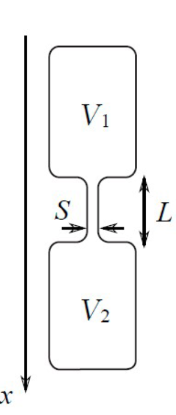
\includegraphics[width=3.5cm]{2.2.1_1}
	\caption{Общая схема установки}
	\label{ris1}
\end{wrapfigure}

Важно отметить, что диффузия -- относительно медленный процесс, и для его наблюдения необходимо отсутствие конвекции, т. е. макроскопических течений газа. Для этого необходимо обеспечить равенство давлений и температур в сосудах до начала измерений.

В общем случае концентрации компонентов $ n(t, x) $ зависят от как от координаты, так и времени. Задача упрощается, если объём соединительной трубки мал по сравнению с объёмами сосудов -- тогда концентрации газов $ n_1(t) $ и $ n_2(t) $ внутри каждого сосуда можно считать постоянными по всему объёму сосуда, и принять, что процесс выравнивания концентраций происходит благодаря диффузии в трубке.

Рассмотрим подзадачу о диффузии в соединительной трубке. Предположим сперва, что концентрации примеси (гелия) на её торцах поддерживаются постоянными и равными $ n_1 $ и $ n_2 $ соответственно. Тогда через некоторое время в трубке установится стационарный поток частиц, одинаковый в каждом сечении трубки (в противном случае, если бы поток зависел от $ x $, частицы бы накапливались в трубке, и процесс перестал бы быть стационарным). Применяя закон Фика в трубке, получим

\[ j=-D\frac{\partial n}{\partial x} = const \]

Следовательно, распределение концентрации в трубке $ n(x) $ -- линейная
функция:

\begin{equation}
n(x) = \frac{\Delta n}{L} x
\end{equation}
и плотность потока частиц всюду постоянна и равна

\begin{equation}
j=-D\frac{\Delta n}{L},
\end{equation}
где $ \Delta n = n_2-n_1 $ -- разность концентраций гелия на концах трубки.

Теперь вернёмся к процессу выравнивания концентраций в сосудах. Частицы перетекают из сосуда 2 в сосуд 1 по трубке и концентрации $ n_1(t) $ и $ n_2(t) $ меняются во времени. Предположим, что этот процесс происходит достаточно медленно, так что в трубке в любой момент времени успевает установиться практически стационарное течение, описываемое формулами (3), (4). Такое приближение называют квазистационарным. Кроме того, будем считать, что в пределах каждого сосуда частицы распределены равномерно, так что концентрации примеси вблизи трубки и в остальных частях сосуда отличаются мало. Тогда полное число частиц примеси в сосудах равно соответственно $ N_1=n_1V $ и $ N_2=n_2V $. Произведение плотности потока (4) на площадь сечения трубки $ S $ даёт количество частиц, пересекающих в единицу времени любое поперечное сечение трубки. Поэтому

\begin{equation}
\frac{dN_1}{dt}=jS, \quad \frac{dN_2}{dt}=-jS.
\end{equation}
Выразим отсюда скорость изменения $ \Delta n $. Вычитая из второго равенства первое и деля результат на объём сосуда $ V $, с учетом (4) получим

\begin{equation}
\frac{d(\Delta n)}{dt}=-\frac{\Delta n}{\tau},
\end{equation}
где введено обозначение
\begin{equation}
\tau=\frac{1}{D}\frac{VL}{2S}.
\end{equation}

Интегрируя (6), получаем, что разность концентраций будет убывать по экспоненциальному закону

\begin{equation}
\Delta n = \Delta n_0 e^{-t/\tau},
\end{equation}
где $ \Delta n_0 $ -- разность концентраций примеси в сосудах в начальный момент времени. Видно, что величина $ \tau $ есть характерное время выравнивания концентраций между сосудами. Оно определяется геометрическими размерами установки и коэффициентом диффузии.

Отметим, что для применимости квазистационарного приближения необходимо убедиться, что время процесса $ \tau $ много больше характерного времени диффузии отдельной частицы вдоль трубки $ L $, которое согласно закону Эйнштейна–Смолуховского по порядку величины равно

\begin{equation}
\tau_\text{диф} \sim L^2/2D.
\end{equation}

Кроме того, если сосуды расположены вертикально, может возникнуть вопрос о влиянии силы тяжести на диффузию. Влиянием гравитации можно пренебречь, если перепад потенциальной энергии в сосуде много меньше энергии теплового движения частиц $ mgh \ll kT $. Нетрудно проверить, что для молекулярной диффузии в нашем эксперименте это выполняется с большим запасом.

\subsection{Методика измерений}

Для измерения разности концентраций в установке применяются датчики теплопроводности. При этом используется тот факт, что теплопроводность $ \kappa $ смеси зависит от её состава. В общем случае зависимость $ \kappa(n) $ довольно сложна, однако при малой разности $ \Delta n $ концентраций в сосудах можно ожидать, что разность теплопроводностей будет изменяться прямо пропорционально $ \Delta n $:

\[ \Delta \kappa = \kappa(n_2)-\kappa(n_1)\approx\text{const}\cdot\Delta n. \]

Эксперименты показывают, что если доля примеси гелия составляет менее
15\%, отклонение от линейной зависимости не превышает 0,5\%, что для наших целей вполне достаточно.

Сами датчики теплопроводности устроены следующим образом. Тонкая платиновая проволочка, протянутая вдоль оси стеклянного цилиндра, нагревается током. Внутренняя полость датчика сообщается с объёмом камеры через отверстия, размеры которых таковы, что скорость диффузии из объёма сосуда в полость датчика значительно больше скорости диффузии из одного объёма в другой. Таким образом, состав газа в датчике практически совпадает с составом газа в объёме. Тепло от проволочки к стенке цилиндра передаётся главным образом за счёт теплопроводности газа, находящегося внутри цилиндра. При заданной мощности нагревания приращение температуры проволочки и, следовательно, приращение её сопротивления пропорциональны теплопроводности газа.

Для измерения сопротивлений используется мостовая схема, позволяющая определять разность показаний датчиков с высокой точностью. Мост балансируется при заполнении сосудов (и датчиков) одной и той же смесью. При заполнении сосудов смесями различного состава возникает <<разбаланc>> моста. При незначительном различии в составах смесей показания вольтметра, подсоединённого к диагонали моста, будут пропорциональны разности концентраций примеси: $ U\propto\Delta\kappa\propto\Delta n $. В процессе диффузии разность концентраций убывает по закону (8), и значит по тому же закону изменяется напряжение:

\begin{equation}
U=U_0e^{-t/\tau},
\end{equation}
где $ U_0 $ -- показание гальванометра в начальный момент времени. Измеряя экспериментально зависимость $ U(t) $, можно получить характерное время
процесса $ \tau $, откуда по формуле (7) определить коэффициент диффузии $ D $.

\begin{figure}[htbp]
	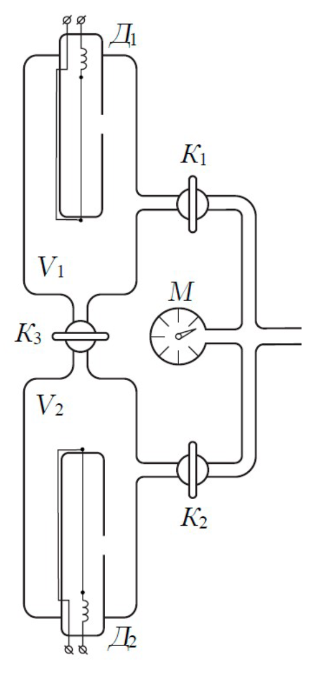
\includegraphics[width=55mm]{2.2.1_2}
	\hfill
	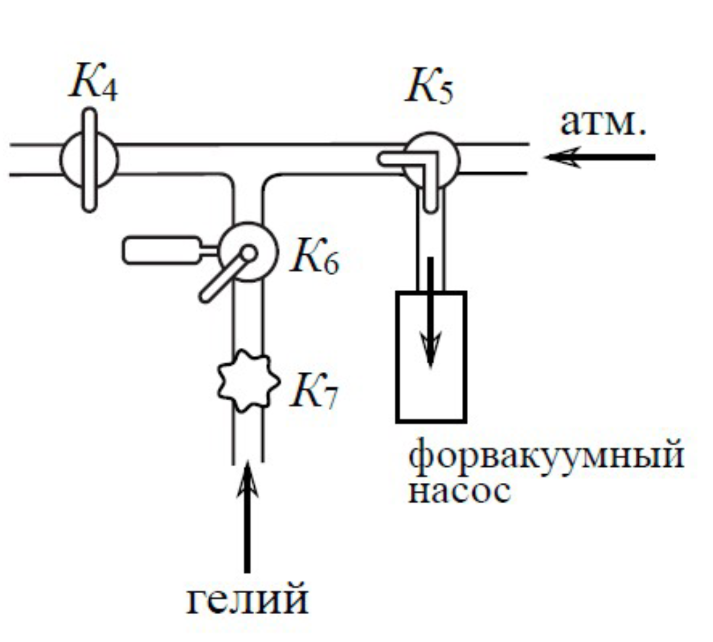
\includegraphics[height=110mm]{2.2.1_3}\\
	\parbox{55mm}{\caption{Измерительная часть установки}\label{ris2}}
	\hfill
	\parbox{110mm}{\caption{Конструкция системы откачки}\label{ris3}}
\end{figure}

\subsection{Экспериментальная установка}

Схема измерительной части установки приведена на рис.2. Она соединена с системой откачки и напуска воздуха и гелия. Для откачки используется форвакуумный насос. Конструкции системы откачки и напуска могут быть различны в зависимости от установки; один из вариантов изображен на рис.

Часть установок компьютеризировано, что позволяет записывать зависимость показаний вольтметра $ U(t) $ в реальном времени (на остальных установках фиксация $ U(t) $ ведется вручную с помощью секундомера).

Измерительная часть установки состоит из двух сосудов $ V_1 $ и $ V_2 $, размещённых вертикально. Краны $ K_1 $ и $ K_2 $ служат для управления откачкой и подачей воздуха/гелия в сосуды. Диффузия осуществляется через тонкую короткую трубку, соединяющую сосуды, оснащённую краном $ K_3 $. К соединительным трубкам подключен манометр M, измеряющий разность давлений между соединительными трубками и атмосферой, и позволяющий измерять давления в разных частях системы (в зависимости от положения кранов).

Выравнивание давлений в сосудах $ V_1 $ и $ V_2 $ без изменения состава газов в них может быть осуществлено через обводные трубки посредством кратковременного открытия кранов $ K_1 $ и $ K_2 $ (при закрытом $ K_3 $).

\begin{wrapfigure}{r}{5cm}
	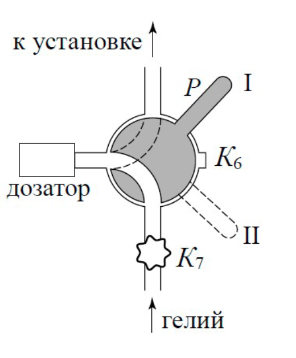
\includegraphics[width=5cm]{2.2.1_4}
	\caption{Механизм подачи гелия}
	\label{ris4}
\end{wrapfigure}

Гелий содержится в баллоне (не изображен на рис.) под давлением, превышающим атмосферное. Для предотвращения избыточного расхода гелия и его неконтролируемого проникания в установку предусмотрен металлический кран $ K_7 $, отделяющий её от баллона с гелием. Его открывают только на время непосредственного заполнения установки гелием, остальное время он должен быть закрыт. Для подачи малых порций гелия предусмотрен двухходовый кран с дозатором (рис. \ref{ris4}). При повороте рычажка $ P $ в положение $ I $ гелий в небольшом количестве поступает в дозатор (если открыт $ K_7 $), а при повороте $ P $ в положение $ II $ порция из дозатора поступает в установку.

Датчики теплопроводности Д$ _1 $ и Д$ _2 $, расположенные в сосудах $ V_1 $ и $ V_2 $ соответственно, включены в мостовую электрическую схему согласно рис. В одну из диагоналей моста включён высокочувствительный вольтметр (гальванометр) Г, к другой подключается источник небольшого постоянного напряжения. Сопротивления проволок датчиков составляют одно из плеч моста. Второе плечо составляют переменные сопротивления $ R_1 $, $ R_2 $ и $ R $, служащие для установки показаний вольтметра Г на нуль (балансировка моста). Сопротивления $ R_1 $ и $ R_2 $ спарены (их подвижные контакты находятся на общей оси) и изменяются одновременно при повороте ручки грубой регулировки. Точная балансировка выполняется потенциометром $ R $. Балансировку необходимо проводить перед каждым экспериментом заново: при этом установка заполняется чистым газом (воздухом без гелия) при давлении, близком «рабочему» (при котором затем будут проводится измерения).

\begin{figure}[H]
	\begin{center}
		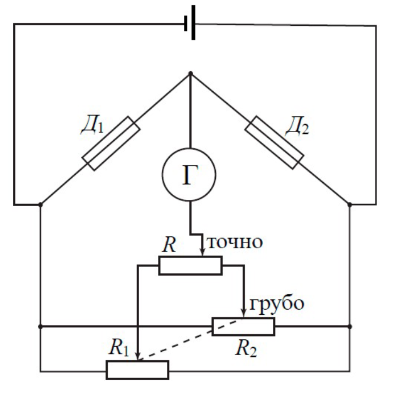
\includegraphics[width=7cm]{2.2.1_5}
	\end{center}
	\caption{Схема мостовой схемы}
	\label{ris5}
\end{figure}

\section{Результаты измерений и обработка данных}

\subsection{Измерение коэффициента взаимной диффузии в зависимости от давления}

Для смеси гелий-воздух исследуем зависимость коэффициента взаимной диффузии о начального давления в системе. Для этого будем фиксировать с помощью компьютера в лаборатории зависимость показаний вольтметра от времени, прошедшего с начала эксперимента. Полученные результаты заносим в таблицу. По полученным результатам нарисуем графики зависимости напряжения от времени в обычном логарифмическом масштабах по оси ординат.:

\begin{figure}[H]
	\begin{center}
		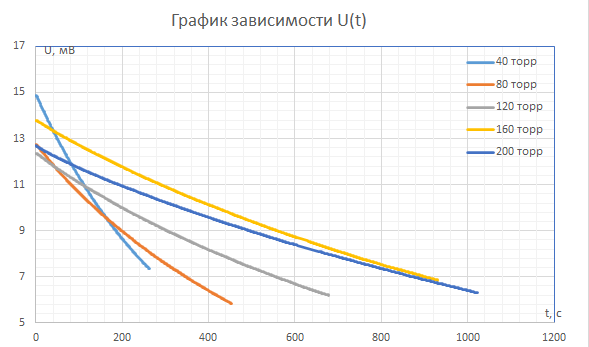
\includegraphics[width=14cm]{2.2.1_gr_1}
	\end{center}
	\label{ris6}
\end{figure}


\begin{figure}[H]
	\begin{center}
		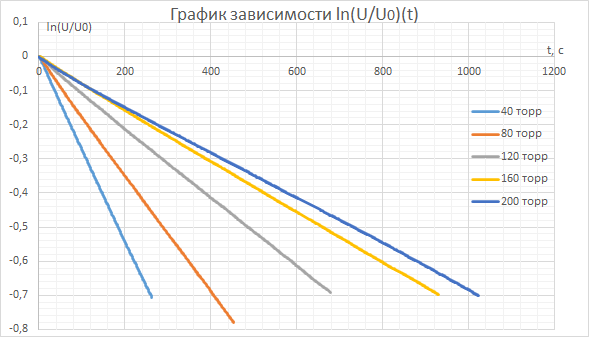
\includegraphics[width=14cm]{2.2.1_gr_2}
	\end{center}
	\label{ris7}
\end{figure}

\begin{equation}
\alpha=\frac{<t\ln (U/U_{0})>}{<t^2>}
\end{equation}

\begin{equation}
\sigma^\text{случ}_{\alpha} = \sqrt{\frac{1}{N-2} \frac{<\ln (U/U_{0})>^2}{<t>^2} - {\alpha}^2},
\end{equation}
где N -- колличество измерений. При этом можно считать, что $ \sigma_B \approx \sigma_B^\text{случ} $, т.к. показания вольтметра довольно точны и систематическая ошибка мала по сравнению со случайными флуктуациями напряжения в ходе эксперимента.

Проводя данные вычисления для каждого значения, заносим результаты в таблицу. Из (10) получаем, что $\tau=-\alpha^{-1}$. При этом погрешность \[ \sigma_\tau = \tau \cdot \frac{\sigma_{\alpha}}{|\alpha|}. \]

\begin{table}[H]
	\centering
	\begin{tabular}{|c|c|c|c|c|c|}
		\hline
		P, торр & $\sigma_{P}$, торр & $\alpha, c^{-1}*10^{-3}$ & $\sigma_{\alpha}, c^{-1} * 10^{-3}$ & $\tau$, c & $\sigma_{\tau}, c$ \\ \hline
		40 & 0.53 & -2,710 & 0.009 & 369.0 & 1.2 \\ \hline
		80 & 0.53 & -1,729 & 0.007 & 578.0 & 2.3 \\ \hline
		120 & 0.53 & -1,029 & 0.004 & 970.9 & 3.8 \\ \hline
		160 & 0.53 & -0,758 & 0.003 & 1315.8 & 5.2 \\ \hline
		200 & 0.53 & -0,688 & 0.003 & 1449.3 & 6.3 \\ \hline
	\end{tabular}
\end{table}

Вычисляем эти параметры и результаты также заносим в таблицу . Dыразим коэффициент взаимной диффузии: \begin{equation}
 D = \frac{1}{\tau}\cdot\frac{VL}{2S},
\end{equation} где параметры $ V $ и $ L/S $ определяются лишь геометрическими параметрами установки, и в данном случае равны: $ V = (1,20 \pm 0,03)*10^{-3} \text{м}^3$, $ L/S = (5.5 \pm 0.5) * 10^2 \text{м}^{-1}$

Таким образом, погрешность вычисление коэффициента взаимной диффузии можно вычислить по следующей формуле:
\[ \sigma_D = D\sqrt{\left(\frac{\sigma_\tau}{\tau}\right)^2+\left(\frac{\sigma_V}{V}\right)^2+\left(\frac{\sigma_{L/S}}{(L/S)}\right)^2}. \]

Используя приведённые выше соотношения, вычисляем коэффициент $ D $ для каждого значения $ P $. Результаты вычислений заносим в таблицу.

\begin{table}[H]
	\centering
	\begin{tabular}{|c|c|c|}
		\hline
		P, торр & D, $\frac{\text{м}^2}{c} * 10^{-4}$ & $\sigma_{D}\frac{\text{м}^2}{c} * 10^{-4}$ \\ \hline
		40 & 8.9 & 0.8 \\ \hline
		80 & 5.7 &  0.5\\ \hline
		120 & 3.4 & 0.3 \\ \hline
		160 & 2.5 & 0.2 \\ \hline
		200 & 2.3 & 0.2 \\ \hline
	\end{tabular}
\end{table}

\subsection{Экстраполяция к атмосферному давлению}

Экстраполируем полученные в 6.1 результаты к атмосферному давлению. Для этого построим график зависимости $ D(1/P) $. Подготовим необходимые для построения данные, занесём их в таблицу, затем построим график.

\begin{table}[H]
	\centering
	\begin{tabular}{|c|c|c|c|}
		\hline
		$P^{-1}, \text{торр}^{-1} * 10^{-3}$ & $\sigma_{P}, \text{торр}^{-1} * 10^{-3}$ & D, $\frac{\text{м}^2}{c} * 10^{-4}$ & $\sigma_{D}\frac{\text{м}^2}{c} * 10^{-4}$ \\ \hline
		25.0 & 0.3 & 8.9 & 0.8 \\ \hline
		12.50 & 0.08 & 5.7 & 0.5 \\ \hline
		8.33 & 0.04 & 3.4 & 0.3 \\ \hline
		6.25 & 0.02 & 2.5 & 0.2 \\ \hline
		5.00 & 0.01 & 2.3 & 0.2 \\ \hline
	\end{tabular}
\end{table}

\begin{figure}[H]
	\begin{center}
		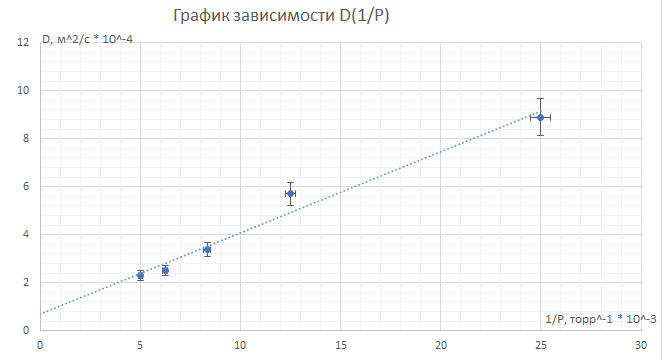
\includegraphics[width=14cm]{2.2.1_gr_3}
	\end{center}
	\label{ris8}
\end{figure}

У полученного графика по МНК определим коэффициенты k и b (прямая задаётся уравнением y = kx + b)

$k = 3.4 * 10^{-2} \frac{\text{м}^2}{c * \text{торр}}$ \;\;\;\;\; $\sigma_{k} = 0,3 * 10^{-2} \frac{\text{м}^2}{c * \text{торр}}$ 

$b = 7*10^{-5} \frac{\text{м}^2}{c}$ \;\;\;\;\; $\sigma_{b} = 4*10^{-5} \frac{\text{м}^2}{c}$

Ввиду малости значения b, можно считать подтвержденной модель соотношения D и P, а значит пересчитаем значение k, зная, что b = 0

$k = (3.8 \pm 0.3) * 10^{-2} \frac{\text{м}^2}{c * \text{торр}}$

Согласно полученным данным, для атмосферного давления (760 торр) коэффициент диффузии D будет равен $(5.0 \pm 0.4)*10^{-5} \frac{\text{м}^2}{c}$

\subsection{Вычисление длины свободного пробега атомов гелия в воздухе и эффективного сечения столкновений атомов гелия с молекулами воздуха}

По полученным в 6.2 данным вычислим длину свободного пробега $ \lambda $ атомов гелия в воздухе. Согласно (2):

\[ D = \frac{1}{3}\lambda \overline{v} = \frac{1}{3}\lambda\sqrt{\frac{8RT}{\pi\mu}}. \]

Отсюда получаем следующее:

\[ \boxed{\lambda = 3D\sqrt{\dfrac{\pi\mu}{8RT}} \approx (120 \pm 10) \text{ нм}}\]

Используя длину свободного пробега, можно оценить сечение столкновения атомов гения с молекулами воздуха $ \sigma $ по следующей формуле:

\[ \sigma = \frac{1}{n_\text{возд}\lambda}, \]

где $ n_\text{возд} \approx 2,65 \cdot 10^{25} $ м$ ^{-3} $ -- концентрация воздуха при нормальных условиях. Производя расчёты, получаем:

\[ \boxed{\sigma \approx (3,1 \pm 0,3) \cdot 10^{-19} \text{ м}^2}\]

\section{Обсуждение результатов и выводы}
В ходе работы были достигнуты следующие цели:
\begin{itemize}
\item Зафиксирована зависимость концентрации гелия в воздухе от времени
\item Экспериментально подтверждены теоретические зависимости, полученные ранее
\item Определён коэффициент взаимной диффузии системы гелий-воздух, а также оценены значения длины свободного пробега молекулы гелия и эффективного сечения столкновения молекул гелия и воздуха
\end{itemize}

Значение коэффициента диффузии $D = (5.0 \pm 0.4)*10^{-5} \frac{\text{м}^2}{c}$ получено с точностью 8\%, причем основной вклад внесли погрешности измерения геометрических характеристик системы, что говорит о необходимости увеличения точности методов.

Табличное значение равно $6.2 * 10^{-5} \frac{\text{м}^2}{c}$, что не лежит в пределах погрешности наших измерений. Это говорит о необходимости повторения эксперимента с повторными измерениями для увеличения вероятности нахождения истинного значения, а также более точной настройки оборудования

Значения длины свободного пробега \[ \boxed{\lambda = 3D\sqrt{\dfrac{\pi\mu}{8RT}} \approx (120 \pm 10) \text{ нм}}\] и эффективного сечения столкновения молекул гелия и воздуха \[ \boxed{\sigma \approx (3,1 \pm 0,3) \cdot 10^{-19} \text{ м}^2}\] получены \%. Т.к. это косвенно полученные величины, то методы увеличения точности будут совпадать с предложенными для коэффициента диффузии.

Табличное значение длины свободного пробега молекулы гелия в воздухе равно 175нм, что не укладывается в нашу погрешность. Однако систематическое (относительно небольшое) отклонение двух полученных величин позволяет говорить о том, что основной вклад в это внесло отклонение условий проведения эксперимента от нормальных.

\end{document}